\documentclass{article}
\usepackage[utf8]{inputenc}
\usepackage{graphicx}
\usepackage{epstopdf}
\usepackage{caption}
\usepackage{subcaption}
\usepackage{multirow}
\usepackage{hyperref}
\usepackage{url}
\usepackage{seqsplit}
\hypersetup{pdfstartview={FitH null null null}}
\usepackage{amssymb,amsmath}
\usepackage{amsthm}
\usepackage{empheq}
\usepackage{algorithm,algpseudocode}
\usepackage[margin=1.5in]{geometry}
\usepackage{listings}
\usepackage{program}
\lstset{language=Python} 

\usepackage{listings}
\usepackage{color} %red, green, blue, yellow, cyan, magenta, black, white
\definecolor{mygreen}{RGB}{28,172,0} % color values Red, Green, Blue
\definecolor{mylilas}{RGB}{170,55,241}


\title{Comparison of protein-protein docking prediction and optimization methods}
\author{Caiwei Wang, Xiaokai Qian, Sean Lander, \\Haipei Fan, Puneet Gaddam, Brett Koonce\\\\University of Missouri - Columbia}

\date{April 7, 2014}

\algloopdefx{NoEndIf}[1]{\textbf{If} #1 \textbf{then}}

\begin{document}

\maketitle

\section{Abstract}

In this paper we applied three docking tools (Zdock, Cluspro and Hex) to two CAPRI targets (T50 and T53), improved prediction accuracy using docking optimization and assessed the performance using a few complementary tools (RosettaDock and RMSD). We first selected the receptor and ligand PDBs of T50 and T53. After pre-processing we created decoys using Zdock, Cluspro and Hex, and then scored and optimized them using RosettaDock. We then compared the results between before and after optimization by measuring both their RosetttaDock scores and the RMSD of the docking interface. We used these results to analyze performance across the tools we used in order to better understand the tools and how they may complement or hinder one another. Ultimately, we visualized the top model from each decoy group.

\section{Introduction}

Protein-protein docking is used to predict the structure of a protein complex given a receptor and a ligand. It is very useful in drug creation and disease prevention. Because the computational power needed for predictions can be high, many unique algorithms and methods have been created to both predict and score docked structures.

For this method comparison we will be using three prediction servers, each of which use a variation on the Fast Fourier Transform method for prediction and their own unique methods for rankings. We then standardize these predictions using RosettaDock's scoring function. Once the top 10 are selected we will apply Rosetta's optimization method, which allows for a relaxing of side-chain constraints, before scoring and sorting them a second time. We will then use RMSD, a traditional scoring method when native conformation is known, of the predicted interface in order to analyze and compare the different methods of prediction, optimization, and scoring.

\section{Methods}



\subsection{Pipeline}

\begin{figure}[H]
\begin{center}
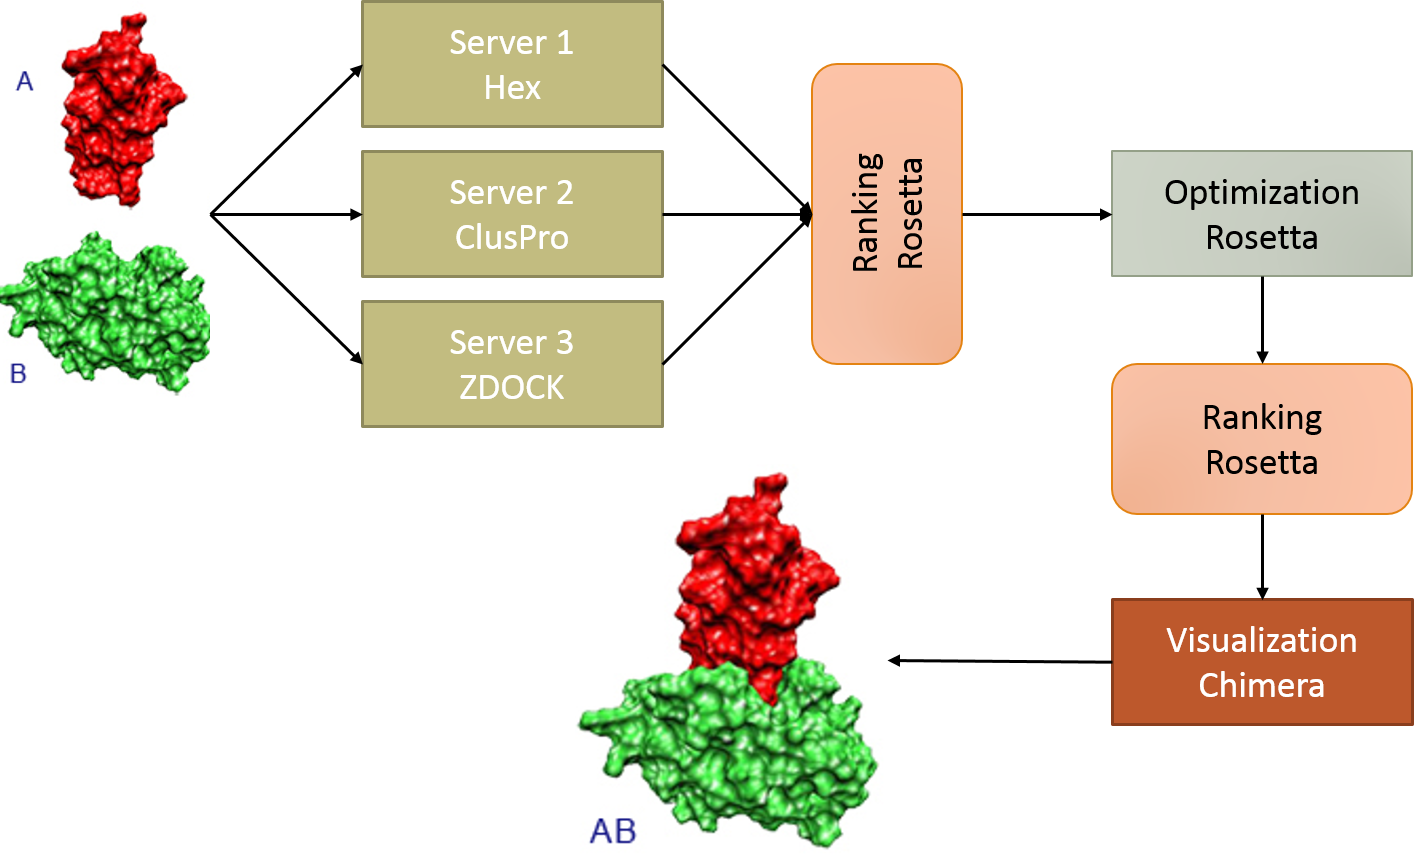
\includegraphics[width=\textwidth]{pipeline}
\caption{An overview of the comparison pipeline}
\label{Fig:blosum}
\end{center}
\end{figure}

\begin{enumerate}
\item Decoy Creation:
Decoys are created using an ensemble of docking servers. This list can be extended beyond the servers listed, as well as include locally created predictions.

\item Ranking:
RosettaDock's prediction scoring is used to normalize the results, as each tool uses its own scoring and ranking system. The decoys are then ranked based on their new scores and the top 10 continue on for optimization.

\item Optimization:
Once again RosettaDock is used, this time for its optimization capabilities. The top 10 decoys are fed into Rosetta and the results are fed into a second round of scoring.

\item Final Selection and Scoring:
The optimized decoys are scored by RosettaDock once again and ranked accordingly. The top scoring model is chosen as the best candidate.

\item Visualization:
Chimera is used to visualize the best model overlaid with the native conformation, as well as the top 10 before and after optimization.
\end{enumerate}

\subsection{CAPRI Target and Docking Tool Selection}

We selected the following template-free targets from the CAPRI database to build a model for: T53, T50. These targets were chosen due to their high predictability by many of the tools used, allowing for a balanced comparison of predictive capacity on easy targets.

The tools selected represent some of the different methods currently employed for docking prediction and rankings - Fast Fourier Transforms, Spherical Polar Fourier, filter by clustering and data-driven rankings - as well as how base decoys compare to their optimized counterparts. 

\subsection{Pre-Processing}

In our project, we choose T50 and T53 as our targets. In T50, the given initial file contains all receptor and ligand information, so we need spilt them into two pdb files so that we can dock them. Chain A and B are the structure of the receptor and Chain C is the structure of ligand. As for T53, CAPRI only provides the structure of receptor. We are given the sequence of the ligand, so we have to predict the structure before we can dock them. In our project, we predicted the structure of ligand of T53 by MuFold server. 


\subsection{Decoy Creation}



\subsubsection{Hex}

    Hex server is the first Fourier transform (FFT)-based protein docking server to be powered by graphics processors. Using two graphics processors simultaneously, a typical 6D docking run takes approximately 15 s, which is up to two orders of magnitude faster than conventional FFT-based docking approaches using comparable resolution and scoring functions. The server requires two protein structures in PDB format to be uploaded, and it produces a ranked list of up to 1000 docking predictions. Knowledge of one or both protein binding sites may be used to focus and shorten the calculation when such information is available. The first 20 predictions may be accessed individually, and a single file of all predicted orientations may be downloaded as a compressed multi-model PDB file. The server is publicly available and does not require any registration or identification by the user.

\subsubsection{ClusPro}

ClusPro is a web server which uses an automated rigid-body docking and discrimination algorithm that rapidly filters docked conformations, and ranks them based on their clustering properties. 

After signing up for an account and logging into the server, you can create a docking job with a receptor and ligand by uploading the PDB files of T50 and T53. You may optionally choose what chains to use in docking. After that, you can view the queue status for the decoys completed. It will generate the number of top models you choose.

\subsubsection{ZDOCK}

ZDOCK uses a mixture of Fast Fourier Transform and data-driven scoring/ranking in order to create and sorts its decoy. While this allows for very fast decoy creation, it results in a stochastic algorithm, so multiple runs will always generate the same results. The ZDOCK server produces 500 decoys on a run, but only the top 10 of those are available for download, making it hard to build up an appropriately sized sample group.

\subsection{Decoy Optimization}

\begin{enumerate}

\item Decoy Ranking

\item Optimization

\end{enumerate}



\section{Results}



\subsection{Interface Creation}

While we can (and do) score the combined protein strands as a whole, we would also like to score only those regions of the proteins that are in contact, better known as the interface.  In order to do this, we wrote script that did the following:\\

\begin{program}
  \FOR i:=1 \TO length(chainA) \STEP 1 \DO
	a := PDB[ATOM[i]]
    \FOR j:=1 \TO length(chainB) \STEP 1 \DO
	b := PDB[ATOM[j]
    \IF (distance(a,b) < 5 angstrom) \DO
addToListOfInterfaceResidues(RESIDUE[a], RESIDUE[b])
    \END
   \END
\END
\end{program}

Then, we simply create a copy of the original PDB file using only the residues in our interface list for the purposes of scoring.  Our actual code is slightly different than the above.  First, we initially build a k-d tree of the locations of each atom in our target protein in order to speed up the distance search process significantly.  Second, we use a unique set for our collection of interface residues in order to avoid duplicate effort.\\

Finally, we simply run this script on each candidate PDB file in order to generate a collection of interface decoys for scoring.

\subsection{Scoring Methods - RMSD vs RosettaDock}

\begin{enumerate}

\item Before Optimization



\item After Optimization



\end{enumerate}

\subsection{Visualization}



\section{Evaluation}

\subsection{Non-optimized scores}

After we generate decoys from three servers, we pick the best decoy as our evaluation target. We use TM-score and RMSD(overall) as our score functions. The following are our two result tables:

\begin{center}
\begin{tabular}{|l|c|c|c|r|}
\multicolumn{4}{c}{T50} \\
    \hline
      & ClusPro & ZDock & Hex \\ \hline
    TM-Score & 0.9941 & 0.1490 & 0.9941 \\ \hline
    RMSD & 0.541 & 25.304 & 0.514 \\
    \hline
    \end{tabular}
\end{center}

\begin{center}
\begin{tabular}{|l|c|c|c|r|}
\multicolumn{4}{c}{T53} \\
    \hline
      & ClusPro & ZDock & Hex \\ \hline
    TM-Score & 0.2418 & 0.8420 & 0.2418 \\ \hline
    RMSD & 8.712 & 16.637 & 8.712 \\
    \hline
    \end{tabular}
\end{center}


\subsection{Optimized scores}

After that, we used Rosettadock to optimize our decoys from three servers. Since the format of ZDock results is not acceptable for Rossettadock, we only optimize decoys of Hex and Cluspro. The next two table show these results (we only present the top structure). Very interesting, there is no improvement. We may figure out this problem in further work.

\begin{center}
\begin{tabular}{|l|c|c|c|r|}
\multicolumn{3}{c}{T50} \\
    \hline
      & ClusPro & Hex \\ \hline
    TM-Score & 0.9941 & 0.9941 \\ \hline
    RMSD & 0.514 & 0.514 \\
    \hline
    \end{tabular}
\end{center}

\begin{center}
\begin{tabular}{|l|c|c|c|r|}
\multicolumn{3}{c}{T53} \\
    \hline
      & ClusPro & Hex \\ \hline
    TM-Score & 0.2418 & 0.2418 \\ \hline
    RMSD & 8.712 & 8.712 \\
    \hline
    \end{tabular}
\end{center}




\subsection{Interface scores}

Since overall rmsd can not reflect the quality of the complex very well, we tried to compare the interfaces of decoys with the one of native structure. The next two tables show results. From these two tables, they indicate that good overall RMSD can’t promise a good interface structure.


\begin{center}
\begin{tabular}{|l|c|c|c|r|}
\multicolumn{4}{c}{T50} \\
    \hline
      & ClusPro & ZDock & Hex \\ \hline
    TM-Score & 0.1890 & 0.0291 & 0.1920 \\ \hline
    RMSD & 0.328 & 20.319 & 0.334 \\
    \hline
    \end{tabular}
\end{center}


\begin{center}
\begin{tabular}{|l|c|c|c|r|}
\multicolumn{4}{c}{T53} \\
    \hline
      & ClusPro & ZDock & Hex \\ \hline
    TM-Score & 0.0592 & 0.0979 & 0.0557 \\ \hline
    RMSD & 2.894 & 3.854 & 3.858 \\
    \hline
    \end{tabular}
\end{center}





\section{Citations}

We thank the following tools and papers: \\\\



\end{document}
